\chapter{Interferometry and Refractive Diagnostics}
\label{ch:interf}

Every diagnostic in the preceding chapters — electrostatic probes, laser-induced fluorescence, optical emission spectroscopy — infers the electron density $n_{\mathrm{e}}$ either from a current--voltage characteristic that perturbs the local plasma, or from a line-shape or line-ratio model depending on an assumed electron energy distribution and collisional--radiative balance. Interferometry is complementary: it measures the phase delay imposed on an electromagnetic probe beam by the free electrons, following directly from the cold-plasma dispersion relation with no dependence on electron energy distribution, immersed surface, or atomic model. Because the measured phase shift is a line integral of $n_{\mathrm{e}}$ along the probe chord, it delivers an absolute, model-independent, non-perturbing constraint on electron density with sub-microsecond time resolution \cite{ref0391}. This chapter develops the refractive-index physics underlying the technique, describes the principal architectures — Mach--Zehnder, heterodyne, multi-chord, and two-colour dispersion interferometry — and closes with its role in quantifying ion energy flux across the plasma sheath: a fast, assumption-free constraint against which sheath models and the other diagnostics of this monograph can be calibrated.

\section{Plasma Refractive Index and Its Dependence on Electron Density}
\label{sec:interf-refractive}

\subsection{Cold-Plasma Dispersion and the Refractive Index}

The propagation of a transverse electromagnetic wave of angular frequency $\omega$ through an unmagnetized, collisionless plasma is governed by the dielectric function
\begin{equation}
\varepsilon(\omega) = 1 - \frac{\omega_{\mathrm{pe}}^{2}}{\omega^{2}}, \qquad
\omega_{\mathrm{pe}}^{2} = \frac{n_{\mathrm{e}} e^{2}}{\varepsilon_{0} m_{\mathrm{e}}},
\label{eq:eps-omega}
\end{equation}
where $\omega_{\mathrm{pe}}$ is the electron plasma frequency, $e$ the elementary charge, $\varepsilon_{0}$ the vacuum permittivity, and $m_{\mathrm{e}}$ the electron mass; the ion contribution, smaller by the mass ratio, is neglected. The refractive index follows from $k^{2}c^{2} = \omega^{2}\varepsilon(\omega)$,
\begin{equation}
n_{\mathrm{r}}(\omega) = \sqrt{\varepsilon(\omega)} = \sqrt{1 - \frac{\omega_{\mathrm{pe}}^{2}}{\omega^{2}}}.
\label{eq:nr-exact}
\end{equation}
For every interferometric configuration of interest, $\omega \gg \omega_{\mathrm{pe}}$, so this expands to leading order,
\begin{equation}
n_{\mathrm{r}}(\omega) \approx 1 - \frac{1}{2}\frac{\omega_{\mathrm{pe}}^{2}}{\omega^{2}}
= 1 - \frac{e^{2}}{2\varepsilon_{0} m_{\mathrm{e}} \omega^{2}}\, n_{\mathrm{e}}.
\label{eq:nr-approx}
\end{equation}
Two properties matter: $n_{\mathrm{r}} < 1$, so the probe beam is advanced in phase rather than retarded; and the departure from unity is linear in $n_{\mathrm{e}}$, underlying both the simplicity of the inversion problem (Section~\ref{sec:interf-multichord}) and the small beam refraction at low density.

\subsection{Critical Density and Wavelength Selection}

Equation~\eqref{eq:nr-exact} shows $n_{\mathrm{r}}$ vanishes, and the wave can no longer propagate, when $\omega = \omega_{\mathrm{pe}}$. The corresponding \emph{critical density} $n_{\mathrm{c}}$ follows by setting $\omega_{\mathrm{pe}}=\omega=2\pi c/\lambda$ in Eq.~\eqref{eq:eps-omega}:
\begin{equation}
n_{\mathrm{c}} = \frac{4\pi^{2}\varepsilon_{0} m_{\mathrm{e}} c^{2}}{e^{2}\,\lambda^{2}}
\;\approx\; \frac{\SI{1.117e27}{\per\cubic\meter}}{\left(\lambda/\si{\micro\meter}\right)^{2}}.
\label{eq:ncrit}
\end{equation}
This sets a hard upper bound on the density a probe wavelength can traverse: a chord encountering density exceeding $n_{\mathrm{c}}$ is reflected (cut off) rather than transmitted. Together with the phase sensitivity of Section~\ref{sec:interf-phase}, this drives wavelength choice (Table~\ref{tab:wavelengths}). Visible/near-infrared lasers suit dense, laser-produced or pulsed-power plasmas where $n_{\mathrm{e}}$ can exceed $\SI{e26}{\per\cubic\meter}$; CO$_{2}$, FIR, and millimetre-wave sources retain adequate sensitivity in the lower-density plasmas of direct interest to sheath and ion-flux diagnostics \cite{ref0400}.

The derivation assumes an unmagnetized plasma at normal incidence. In a magnetized plasma the dielectric tensor splits into ordinary (O-mode) and extraordinary (X-mode) branches; only the O-mode retains the field-independent form of Eq.~\eqref{eq:nr-approx}, while the X-mode depends explicitly on cyclotron frequency. Probe beams are therefore polarised to couple predominantly to the O-mode, reserving the field-sensitive X-mode (and its Faraday rotation, Section~\ref{sec:interf-vibration}) for dedicated polarimetry.

\section{Phase-Shift Measurement: Mach--Zehnder and Heterodyne Interferometers}
\label{sec:interf-phase}

\subsection{Line-Integrated Phase Shift}

For a probe beam traversing a plasma column of length $L$ along a straight chord $\ell$ — a good approximation whenever refraction (Section~\ref{sec:interf-vibration}) is small — the optical phase accumulated relative to a vacuum path of equal length is
\begin{equation}
\Delta\phi = \frac{\omega}{c}\int_{0}^{L}\bigl[n_{\mathrm{r}}(\ell) - 1\bigr]\,\mathrm{d}\ell
\approx -\frac{\omega}{2c}\int_{0}^{L}\frac{\omega_{\mathrm{pe}}^{2}(\ell)}{\omega^{2}}\,\mathrm{d}\ell,
\label{eq:phase-integral}
\end{equation}
using Eq.~\eqref{eq:nr-approx}. Substituting $\omega_{\mathrm{pe}}^{2}=n_{\mathrm{e}}e^{2}/(\varepsilon_{0}m_{\mathrm{e}})$ and $\omega = 2\pi c/\lambda$ gives the standard working formula of plasma interferometry,
\begin{equation}
|\Delta\phi| = r_{\mathrm{e}}\,\lambda \int_{0}^{L} n_{\mathrm{e}}(\ell)\,\mathrm{d}\ell,
\qquad
r_{\mathrm{e}} \equiv \frac{e^{2}}{4\pi\varepsilon_{0} m_{\mathrm{e}} c^{2}} = \SI{2.818e-15}{\meter},
\label{eq:phase-formula}
\end{equation}
with $r_{\mathrm{e}}$ the classical electron radius. This is the foundation of every technique in this chapter: the raw observable is not $n_{\mathrm{e}}$ itself but $\int n_{\mathrm{e}}\,\mathrm{d}\ell$, multiplied by the single geometric factor $r_{\mathrm{e}}\lambda$ (Table~\ref{tab:wavelengths}; Figure~\ref{fig:phase-vs-density}). Since Eq.~\eqref{eq:phase-formula} contains no free parameters beyond fundamental constants and the known probe wavelength, the inference carries none of the model uncertainty of an assumed electron energy distribution or collisional--radiative balance — the principal advantage over probe or spectroscopic diagnostics.

\begin{table}[htbp]
\centering
\caption{Illustrative phase-shift sensitivity $r_{\mathrm{e}}\lambda$ [Eq.~\eqref{eq:phase-formula}] and cutoff (critical) density $n_{\mathrm{c}}$ [Eq.~\eqref{eq:ncrit}] for probe wavelengths commonly used in plasma interferometry. All entries are computed directly from the analytic cold-plasma dispersion relation; none is a measured value.}
\label{tab:wavelengths}
\begin{tabular}{lcccl}
\toprule
Source / band & $\lambda$ & $r_{\mathrm{e}}\lambda$ (\si{\meter\squared}) & $n_{\mathrm{c}}$ (\si{\per\cubic\meter}) & Typical regime \\
\midrule
He--Ne (visible) & \SI{632.8}{\nano\meter} & \num{1.78e-21} & \num{2.8e27} & dense laser plasma \\
Nd:YAG (near-IR) & \SI{1.064}{\micro\meter} & \num{3.00e-21} & \num{9.9e26} & pulsed-power, dense discharge \\
CO$_{2}$ laser & \SI{10.6}{\micro\meter} & \num{2.99e-20} & \num{9.9e24} & tokamak core, z-pinch \\
FIR (CH$_{3}$OH) & \SI{118.8}{\micro\meter} & \num{3.35e-19} & \num{7.9e22} & fusion edge/core \\
FIR (HCN) & \SI{337}{\micro\meter} & \num{9.50e-19} & \num{9.8e21} & low-density devices \\
Millimetre-wave & \SI{1}{\milli\meter} & \num{2.82e-18} & \num{1.1e21} & processing / low-temperature plasmas \\
\bottomrule
\end{tabular}
\end{table}

\subsection{Mach--Zehnder Configuration}

The most direct realisation of Eq.~\eqref{eq:phase-formula} is the Mach--Zehnder interferometer, in which a coherent beam is split into a probe arm crossing the plasma column and a reference arm of comparable length that does not, the two recombining onto a detector or fringe camera (Figure~\ref{fig:mz-schematic}). Nanosecond- and picosecond-resolved configurations built around frequency-tripled or fourth-harmonic solid-state lasers are standard for dense, transient laser-produced and pulsed-power plasmas, where the short wavelength keeps the critical density well above densities of interest; the local fringe shift at each pixel gives $\Delta\phi(x,y)$ directly, and the density map follows by tomographic inversion (Section~\ref{sec:interf-multichord}).

\begin{figure}[htbp]
\centering
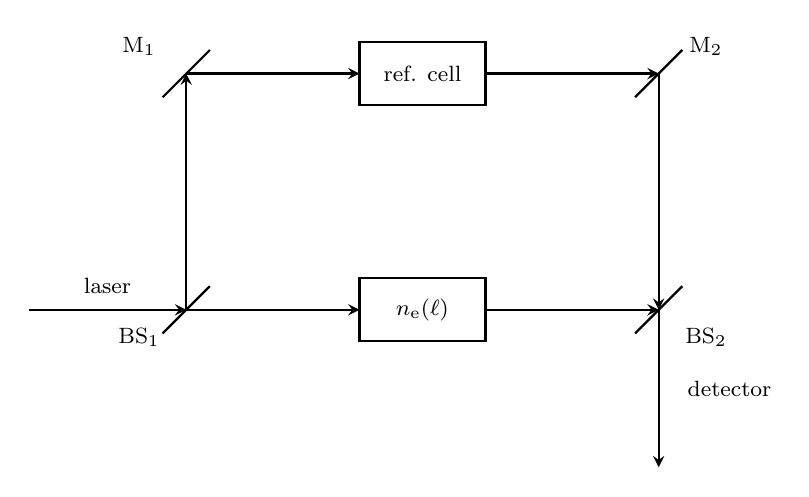
\begin{tikzpicture}[>=stealth, thick]
 \draw[->] (-2,0) -- (0,0);
 \node at (-1,0.3) {\footnotesize laser};
 \draw[->] (0,0) -- (0,3);
 \draw[->] (0,3) -- (2.2,3);
 \draw[->] (3.8,3) -- (6,3);
 \draw[->] (6,3) -- (6,0);
 \draw[->] (0,0) -- (2.2,0);
 \draw[->] (3.8,0) -- (6,0);
 \draw[->] (6,0) -- (6,-2);
 \node at (6.9,-1) {\footnotesize detector};
 \draw (2.2,-0.4) rectangle (3.8,0.4);
 \node at (3.0,0.0) {\footnotesize $n_{\mathrm{e}}(\ell)$};
 \draw (2.2,2.6) rectangle (3.8,3.4);
 \node at (3.0,3.0) {\footnotesize ref. cell};
 \draw (-0.3,-0.3) -- (0.3,0.3);
 \node at (-0.6,-0.35) {\footnotesize BS$_{1}$};
 \draw (-0.3,2.7) -- (0.3,3.3);
 \node at (-0.6,3.35) {\footnotesize M$_{1}$};
 \draw (5.7,2.7) -- (6.3,3.3);
 \node at (6.6,3.35) {\footnotesize M$_{2}$};
 \draw (5.7,-0.3) -- (6.3,0.3);
 \node at (6.6,-0.35) {\footnotesize BS$_{2}$};
\end{tikzpicture}
\caption{Schematic (illustrative, not to scale) layout of a Mach--Zehnder interferometer for line-integrated electron-density measurement. The probe beam traverses the plasma column of density $n_{\mathrm{e}}(\ell)$ along the lower arm; a reference beam of matched nominal optical path length traverses a compensating cell in the upper arm. Beamsplitters BS$_{1}$, BS$_{2}$ and mirrors M$_{1}$, M$_{2}$ recombine the two beams onto a detector, where the resulting fringe pattern encodes the phase difference of Eq.~\eqref{eq:phase-formula}.}
\label{fig:mz-schematic}
\end{figure}

\begin{figure}[htbp]
\centering
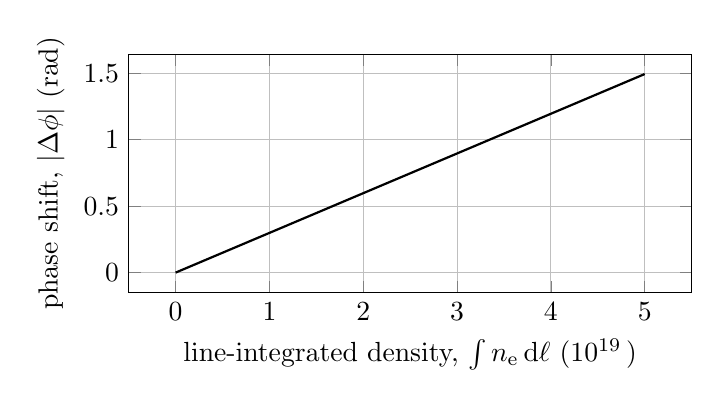
\begin{tikzpicture}
\begin{axis}[
 width=0.72\textwidth,
 height=0.38\textwidth,
 xlabel={line-integrated density, $\int n_{\mathrm{e}}\,\mathrm{d}\ell$ ($10^{19}\,\si{\per\square\meter}$)},
 ylabel={phase shift, $|\Delta\phi|$ (rad)},
 domain=0:5,
 samples=50,
 grid=major,
]
\addplot[black, thick] {0.2987*x};
\end{axis}
\end{tikzpicture}
\caption{Illustrative (analytic, not measured) phase shift at the \SI{10.6}{\micro\meter} CO$_{2}$ line, $|\Delta\phi| = r_{\mathrm{e}}\lambda \int n_{\mathrm{e}}\,\mathrm{d}\ell$ [Eq.~\eqref{eq:phase-formula}], plotted against line-integrated electron density.}
\label{fig:phase-vs-density}
\end{figure}

Because $r_{\mathrm{e}}\lambda$ is fixed once the wavelength is chosen, calibration reduces to accurate knowledge of the probe wavelength — there is no equivalent of the sheath-collection coefficient invoked by a Langmuir probe. The difficulty instead lies in engineering the phase measurement: recovering a phase to a small fraction of one fringe, continuously, despite vibration and detector noise. Homodyne systems address this in part through quadrature (I/Q) detection, combining two interferograms with a fixed $\pi/2$ phase bias to resolve magnitude and sign unambiguously, at the cost of doubled hardware.

\subsection{Heterodyne Detection}

Direct fringe-imaging Mach--Zehnder interferometry recovers $\Delta\phi$ only modulo $2\pi$ and modulo a sign, since a static fringe pattern does not indicate the direction the phase is changing. Heterodyne interferometry removes this ambiguity by imposing a small frequency offset $\Delta f$ between probe and reference beams — via an acousto-optic modulator or Zeeman-split source — so the beams beat continuously at the detector even absent plasma; the plasma-induced shift $\Delta\phi(t)$ modulates this beat signal, demodulated electronically to yield $\Delta\phi(t)$ continuously and unambiguously in sign \cite{ref0400}. It also offers large dynamic range and immunity to slow intensity drifts, since density information is carried by beat phase rather than DC intensity — the architecture of choice for CO$_{2}$-laser and millimetre-wave systems running continuously over a discharge.

\section{Multi-Chord and Dispersion Interferometry: Line-Integrated Density and Inversion}
\label{sec:interf-multichord}

\subsection{Abel Inversion for Cylindrically Symmetric Profiles}

A single chord returns only $\int n_{\mathrm{e}}\,\mathrm{d}\ell$; recovering $n_{\mathrm{e}}(r)$ requires an assumed symmetry or additional chords. For a cylindrically symmetric column and chord of impact parameter $y$, the observable is the Abel transform,
\begin{equation}
S(y) \equiv \int n_{\mathrm{e}}\,\mathrm{d}\ell = 2\int_{y}^{a} \frac{n_{\mathrm{e}}(r)\,r}{\sqrt{r^{2}-y^{2}}}\,\mathrm{d}r,
\label{eq:abel-forward}
\end{equation}
where $a$ is the plasma column radius, inverted analytically by
\begin{equation}
n_{\mathrm{e}}(r) = -\frac{1}{\pi}\int_{r}^{a} \frac{1}{\sqrt{y^{2}-r^{2}}}\,\frac{\mathrm{d}S}{\mathrm{d}y}\,\mathrm{d}y,
\label{eq:abel-inverse}
\end{equation}
which requires the derivative of the chord data with respect to impact parameter — numerically delicate in the presence of noise, so it is normally applied to a smooth fit of $S(y)$ rather than raw data. Abel inversion is exact only for genuinely axisymmetric distributions; departures from symmetry require the multi-chord tomographic approach described next.

\subsection{Multi-Chord Arrays and Tomographic Reconstruction}

Deploying an array of $N$ parallel or fan-shaped chords at distinct impact parameters $y_{i}$ converts Eq.~\eqref{eq:abel-forward} into an overdetermined linear system, $S_{i} = \sum_{j} W_{ij}\, n_{\mathrm{e},j}$, where $W_{ij}$ is a geometric weight matrix encoding the length of chord $i$ within grid cell $j$. This is solved by least-squares, singular-value decomposition, or regularised (Tikhonov) inversion to recover a tomographic density map without invoking symmetry, resolving structure Abel inversion alone cannot. In tokamaks, multi-chord interferometry provides the real-time, line-averaged density signal for feedback control of gas fuelling, its response time being fast compared with actuator timescales \cite{ref0399}.

\subsection{Two-Colour Dispersion Interferometry}

Equation~\eqref{eq:phase-formula} shows $|\Delta\phi| \propto \lambda$: the plasma phase scales as $1/\omega$. A parasitic shift from mechanical vibration instead scales as $\Delta\phi_{\mathrm{vib}} = \omega\,\delta L/c$ for a path-length change $\delta L$ — the opposite dependence. Dispersion interferometry exploits this by probing simultaneously at a fundamental frequency $\omega$ and its second harmonic $2\omega$, generated via a nonlinear crystal, so both colours traverse an identical mechanical path with the same $\delta L$ at every instant:
\begin{align}
\phi(\omega) &= \phi_{\mathrm{pl}}(\omega) + \phi_{\mathrm{vib}}(\omega)
= -\, r_{\mathrm{e}}\lambda \int n_{\mathrm{e}}\,\mathrm{d}\ell \;+\; \frac{\omega\,\delta L}{c}, \\
\phi(2\omega) &= \phi_{\mathrm{pl}}(2\omega) + \phi_{\mathrm{vib}}(2\omega)
= -\, \tfrac{1}{2} r_{\mathrm{e}}\lambda \int n_{\mathrm{e}}\,\mathrm{d}\ell \;+\; \frac{2\omega\,\delta L}{c},
\end{align}
using $\phi_{\mathrm{pl}}(2\omega) = \tfrac{1}{2}\phi_{\mathrm{pl}}(\omega)$ and $\phi_{\mathrm{vib}}(2\omega) = 2\phi_{\mathrm{vib}}(\omega)$. Forming the combination
\begin{equation}
\phi(2\omega) - 2\phi(\omega) = \tfrac{3}{2}\, r_{\mathrm{e}}\lambda \int n_{\mathrm{e}}\,\mathrm{d}\ell,
\label{eq:dispersion-interf}
\end{equation}
the vibration term cancels \emph{exactly}, to all orders in $\delta L$, leaving a signal depending on line-integrated density alone. First developed for large fusion and pulsed-power facilities, this is now standard wherever the mechanical stability of single-colour measurement (Section~\ref{sec:interf-vibration}) cannot be guaranteed \cite{ref0417}.

\section{Vibration Immunity, Wavelength Choice, and Error Sources}
\label{sec:interf-vibration}

\subsection{Sources of Phase Noise and Vibration Compensation}

Because the plasma-induced phase shift is often a small fraction of a fringe, mechanical vibration of mirrors, beamsplitters, windows, and mounts is frequently the dominant noise source, particularly for long-path systems on large devices. A path-length fluctuation $\delta L$ as small as a fraction of the probe wavelength produces a spurious excursion $\Delta\phi_{\mathrm{vib}} = 2\pi\,\delta L/\lambda$ indistinguishable, in single-colour homodyne measurement, from a genuine density change. Differential designs, sharing as much common optical path as possible, suppress uncorrelated vibration noise since a disturbance common to both arms cancels in the phase difference. Where full common-path operation is impractical, retroreflected geometries, active isolation, and, most robustly, the dispersion-cancellation scheme of Eq.~\eqref{eq:dispersion-interf} are used, insensitive to vibration by construction and preferred for pulsed-power interferometry in noisy environments \cite{ref0417}. Heterodyne detection (Section~\ref{sec:interf-phase}) adds a complementary benefit: phase from a continuously running beat signal lets low-frequency vibration appear as slow drift, distinguishable from density fluctuations of interest.

\subsection{Wavelength Trade-offs}

Table~\ref{tab:wavelengths} makes explicit the central trade-off in probe-wavelength selection. Phase sensitivity $r_{\mathrm{e}}\lambda$ increases linearly with wavelength, so long-wavelength sources (CO$_{2}$, FIR, millimetre-wave) are essential whenever line-integrated density is low, as in low-temperature, weakly ionized plasmas. Conversely, critical density falls as $\lambda^{-2}$, so those same wavelengths also suffer beam cutoff first, and are more strongly refracted by transverse gradients, since the bending angle scales with the same $\omega_{\mathrm{pe}}^{2}/\omega^{2}$ factor entering Eq.~\eqref{eq:nr-approx}. Visible and near-infrared sources remain nearly undeflected and immune to cutoff at high density, and are preferred for dense, transient plasmas requiring imaging interferometry \cite{ref0391}.

\subsection{Systematic and Statistical Error Budget}

Table~\ref{tab:errors} summarises further error sources, beyond mechanical vibration, that bound the accuracy of an interferometrically inferred density.

\begin{table}[htbp]
\centering
\caption{Principal error sources in plasma interferometry and their typical mitigation strategies. Entries are qualitative summaries of well-established diagnostic practice, not measured values from a specific experiment.}
\label{tab:errors}
\begin{tabularx}{\textwidth}{@{}l X X@{}}
\toprule
Error source & Typical origin & Mitigation \\
\midrule
Mechanical vibration & Path-length fluctuation of mirrors, windows, optical mounts & Common-path/differential design; two-colour dispersion cancellation; heterodyne detection \\
Fringe-jump ($2\pi$) ambiguity & Rapid density transients exceeding the phase-tracking bandwidth & Heterodyne phase demodulation; sufficient sampling rate; redundant chord comparison \\
Beam refraction & Transverse gradients of $n_{\mathrm{r}}$ steering the beam off the detector aperture & Wide collection optics; retroreflection; correction using measured or modelled gradients \\
Non-plasma dispersion & Vacuum windows, air path, neutral-gas background contributing to phase & Vacuum-referenced calibration shot; evacuated or purged beam path \\
Faraday-rotation crosstalk & Magnetized plasma birefringence coupling into polarization-sensitive optics & Combined polarimetry--interferometry analysis; polarization-insensitive detection \\
Finite detector/electronics bandwidth & Beat-frequency demodulation limited by photodetector or digitizer response & Bandwidth matched to expected $\dot{n}_{\mathrm{e}}$; oversampling \\
Etalon fringes & Parasitic reflections between parallel optical surfaces & Anti-reflection coatings; wedged windows; beam dumps \\
\bottomrule
\end{tabularx}
\end{table}

Fringe-jump ambiguity arises when density changes by more than one fringe within a sampling interval, so the demodulated phase folds back on itself and $\int n_{\mathrm{e}}\,\mathrm{d}\ell$ acquires an integer-fringe offset — a hazard during fast transients, mitigated by adequate sampling bandwidth and cross-checking against adjacent chords. Beam refraction, quantified by the transverse gradient of Eq.~\eqref{eq:nr-approx}, displaces the beam on the detector, potentially causing signal dropout, and imposes a small path-integration error since the ray is no longer exactly the straight chord assumed in Eq.~\eqref{eq:phase-formula}. In magnetized plasmas, birefringence responsible for Faraday rotation couples into any polarization-sensitive element and must be suppressed or exploited deliberately in combined polarimetry--interferometry systems. The non-plasma contribution to the optical path — vacuum windows, residual air, stray gas dispersion — must be removed by a reference phase measurement, since it is otherwise indistinguishable from a genuine plasma shift.

Two subtler contributions complete the budget: low-pass filtering, which attenuates genuine high-frequency structure and so must be validated against the fastest transient of interest; and the statistical noise floor of the recombined beam, which enters the phase measurement additively while the plasma shift enters linearly in density, so the minimum detectable density for a given chord length is the phase resolution divided by $r_{\mathrm{e}}\lambda L$.

\section{Role as a Fast, Robust Density Constraint}
\label{sec:interf-role}

\subsection{Non-Perturbing, Model-Independent Density Measurement}

The defining strength of interferometry, relative to every other diagnostic surveyed in this monograph, is that Eq.~\eqref{eq:phase-formula} is exact for $\omega \gg \omega_{\mathrm{pe}}$ and depends on no property of the electron population beyond its number density: not $T_{\mathrm{e}}$, not the energy-distribution shape, not any collisional--radiative assumption. By contrast, a Langmuir-probe inference requires an assumed sheath-collection model and an immersed electrode that perturbs the plasma sampled, an optical-emission inference requires a full atomic model sensitive to non-Maxwellian departures, and laser-induced fluorescence targets the ion rather than the bulk electron density. Interferometry couples to the plasma only through its linear dielectric response, leaving it undisturbed, with a formula containing no adjustable parameters beyond the known probe wavelength \cite{ref0391} — non-invasiveness and model independence that make it an external constraint against which model-dependent diagnostics, and fluid or kinetic sheath models, can be validated.

\subsection{Coupling to Sheath-Edge Flux Diagnostics}

The ion energy flux delivered to a bounding surface is controlled, in every model developed elsewhere in this monograph, by the density at the sheath edge and the ion speed there, most compactly through the Bohm velocity $u_{\mathrm{B}} = \sqrt{k_{\mathrm{B}} T_{\mathrm{e}}/m_{\mathrm{i}}}$ and a flux $\Gamma_{E} \simeq n_{\mathrm{e}} u_{\mathrm{B}} \overline{E}_{\mathrm{i}}$, where $\overline{E}_{\mathrm{i}}$ is the mean ion impact energy set by the sheath potential drop and the ion velocity distribution $f_{\mathrm{i}}(v)$ at the wall. Every quantity except $n_{\mathrm{e}}$ is set by the local electron temperature and sheath potential profile, so the absolute flux scale is fixed by the density normalization — yet a local probe or spectroscopic measurement near the sheath edge is difficult without perturbing it, and is a point measurement subject to the model dependences noted above. A line-integrated measurement along a chord intersecting the presheath and bulk plasma provides an independent, non-perturbing normalization that, combined with a presheath density-decay profile (Section~\ref{sec:interf-multichord}), can be extrapolated to the sheath edge to give an absolute prediction of $\Gamma_{E}$, resolving density transients too fast for a swept Langmuir-probe characteristic to follow \cite{ref0399,ref0417}.

\subsection{Cross-Validation with Probe and Spectroscopic Diagnostics}

In practice, interferometry rarely operates in isolation: its principal value lies in providing an absolute density benchmark against which Langmuir-probe and collisional--radiative inferences can be cross-checked, and any systematic offset identified. This role is well established in magnetically confined and processing plasmas, where multi-chord interferometry anchors the calibration of faster, more model-dependent point diagnostics; discrepancies with the probe- or spectroscopy-inferred density are themselves diagnostic of departures from assumptions — Maxwellian energy distribution, unperturbed sheath collection, local thermodynamic equilibrium — that alternative techniques must invoke \cite{ref0399}. Multi-wavelength dispersion systems further allow internal validation, since the two-colour combination of Eq.~\eqref{eq:dispersion-interf} and an independent homodyne channel should agree once vibration is accounted for \cite{ref0417}. For this monograph, interferometry supplies the density input without which the ion-energy-flux expressions of the surrounding chapters cannot be placed on an absolute scale.

\subsection{Illustrative Application Domains}

The generality of Eq.~\eqref{eq:phase-formula} means the same logic recurs across plasma regimes, differing chiefly in probe wavelength and vibration-mitigation strategy, while its role as an absolute constraint remains unchanged. In fusion research, multi-chord CO$_{2}$- or FIR-laser interferometry supplies the line-averaged core density for real-time control and absolute normalization of the edge density setting the ion flux to plasma-facing components \cite{ref0399}. In pulsed-power and z-pinch research, fibre-coupled dispersion interferometry provides dynamic, single-shot measurements through the compressing or expanding sheath \cite{ref0417}. In laser-produced plasmas, where densities approach the near-infrared critical density, ultrafast Mach--Zehnder interferometers freeze the evolution on a single shot \cite{ref0391}. In low-temperature processing plasmas — the regime most directly relevant here — millimetre-wave interferometry provides the bulk-plasma density feeding the presheath and sheath without the perturbation risked by an immersed probe \cite{ref0400}. Across every domain, the diagnostic contributes the same quantity, which is why it functions so effectively as a common density reference.

\section{Summary}
\label{sec:interf-summary}

The refractive index of an unmagnetized plasma departs from unity by an amount proportional to electron density, so the phase delay imposed on a transmitted probe beam is a direct, line-integrated, model-independent measure of $n_{\mathrm{e}}$ [Eq.~\eqref{eq:phase-formula}]. Mach--Zehnder interferometers realise this through two-beam interference and fringe imaging, while heterodyne detection removes the sign and fringe-counting ambiguities of static analysis. Multi-chord arrays and tomographic reconstruction convert line-integrated chord measurements into a spatially resolved profile via the Abel-transform relation of Eqs.~\eqref{eq:abel-forward}--\eqref{eq:abel-inverse}, and two-colour dispersion interferometry [Eq.~\eqref{eq:dispersion-interf}] exploits the opposite frequency scaling of the plasma phase shift and vibration noise to cancel the latter exactly. Probe-wavelength selection trades phase sensitivity against beam refraction and critical-density cutoff (Table~\ref{tab:wavelengths}), and a characterised error budget (Table~\ref{tab:errors}) must be applied before a phase measurement becomes an absolute density. Because the result is fast, non-perturbing, and free of the model assumptions required by probe and spectroscopic techniques, interferometry serves as the primary independent normalization for the electron density entering $\Gamma_{E}$, and as the benchmark against which every other diagnostic in this work is tested.
